%#! platex main.tex

%======================================================================
\chapter{評価実験}

本章では, 各食品毎の食事中の音を収集する実験を行う. その後, 収集した音データを分析し, 食事内容および咀嚼回数の推定を行なった.

%----------------------------------------------------------------------
\section{対象とする食事}

図\ref{fig:foods}に示すように, 本研究において対象とする食品は以下の16種類である. 基本的には, 一般的な日本人がよく食べる食品を中心にピックアップしており, 柔らかいものから固いものまで多岐に渡る.

\begin{itemize}
    \item 唐揚げ
    \item ご飯
    \item 味噌汁
    \item サラダ
    \item せんべい
    \item グラタン
    \item クッキー
    \item ポテトチップス
    \item スパゲティ
    \item ヨーグルト
    \item ハンバーグ
    \item サラダチキン
    \item クリームパン
    \item 焼きそば
    \item ゼリー
    \item 焼き魚
\end{itemize}

また録音データの一例として, 図\ref{fig:sample-data}にAirPodsによって計測された録音データの波形を示す.

%----------------------------------------------------------------------
\section{実験準備}

本研究では, Apple社製のAirPodsシリーズ\footnote{AirPods - Apple~\url{https://www.apple.com/jp/airpods/}}を用いて録音を行う. AirPodsシリーズには, AirPodsの第1世代から第3世代, AirPods Proの第1世代から第2世代までのラインナップがあり, 全てのモデルにおいて, 内臓マイクが搭載されている. 評価実験は, 環境音の少ない静かな環境で, 21〜27歳の15名の被験者(\tablename\ref{personaldata})によって行われた. 被験者は, AirPodsを耳に装着し, アプリケーションで測定を開始した上で, 食事を行った. 計測は一品ずつ行い, 食品を変える際は一回計測を終了してから再度計測をしなおすことで, 1つの音データには1種類の食事のみを含むようにした. その結果, 合計13422秒の食事中の録音データを記録することができた. 図\ref{fig:sound-data}は, 食品毎の録音データの録音時間の累計を示す.

\begin{table}[t]
    \centering
    \caption{食品毎の食事内容推定モデルの精度}
    \label{result}
    \scalebox{0.9}{
        \begin{tabular}{c|c|c|c|c}
            \hline
            \textbf{食品} & \textbf{precision} & \textbf{recall} & \textbf{f1-score} & \textbf{support} \\ \hline\hline
            ポテトチップス     & 0.88               & 0.91            & 0.90              & 1409.0           \\ \hline
            クリームパン      & 0.87               & 0.86            & 0.86              & 488.0            \\ \hline
            せんべい        & 0.87               & 0.83            & 0.85              & 1229.0           \\ \hline
            ゼリー         & 0.84               & 0.82            & 0.83              & 512.0            \\ \hline
            スパゲティ       & 0.90               & 0.72            & 0.80              & 454.0            \\ \hline
            サラダ         & 0.76               & 0.81            & 0.79              & 834.0            \\ \hline
            焼きそば        & 0.79               & 0.78            & 0.78              & 556.0            \\ \hline
            クッキー        & 0.80               & 0.75            & 0.77              & 787.0            \\ \hline
            グラタン        & 0.79               & 0.76            & 0.77              & 381.0            \\ \hline
            サラダチキン      & 0.80               & 0.68            & 0.74              & 232.0            \\ \hline
            味噌汁         & 0.75               & 0.69            & 0.72              & 900.0            \\ \hline
            ご飯          & 0.62               & 0.80            & 0.70              & 1170.0           \\ \hline
            ヨーグルト       & 0.68               & 0.64            & 0.66              & 165.0            \\ \hline
            唐揚げ         & 0.67               & 0.57            & 0.62              & 581.0            \\ \hline
            ハンバーグ       & 0.59               & 0.62            & 0.60              & 317.0            \\ \hline
            焼き魚         & 0.54               & 0.54            & 0.54              & 218.0            \\ \hline
        \end{tabular}
    }
\end{table}

\begin{figure}[t]
    \begin{center}
        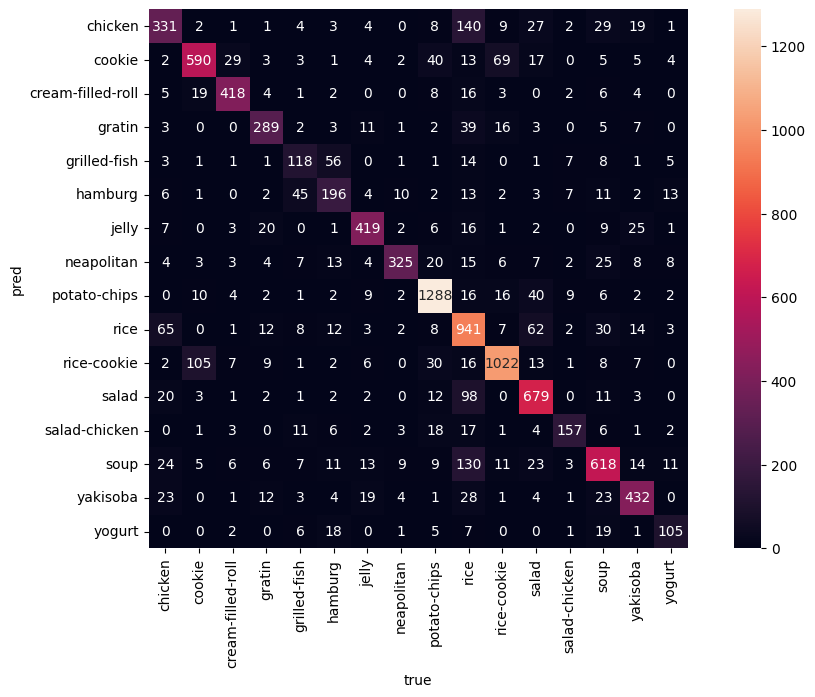
\includegraphics[clip,  width=0.95\hsize]{img/confusion_matrix.png}
        \caption{食事内容推定モデルの混合行列}
        \label{fig:confusion-matrix}
    \end{center}
\end{figure}

%----------------------------------------------------------------------
\section{食事内容の推定}

AirPodsから44100Hzのサンプリング周波数で取得された録音データをスライディングウィンドウで部分時系列データに分割する. その結果, 107421件の音データを得ることができた. ただし, 最大信号強度が$-65dBFS$以下のデータと音の長さが$500ms$に満たないものは除外したため, 最終的に使用したデータは102960件である.

これらのデータを用いて, 食事内容推定モデルを学習させたところ, テストデータに対して, 精度$77.5\%$という結果となった. \tablename\ref{result}に食品毎の精度を示す. F1スコアを比較すると, ポテトチップスが一番精度が高く, 焼き魚が一番精度が低いことがわかる. また, 図\ref{fig:confusion-matrix}に混合行列を示す. 混合行列から, クッキーがせんべいと誤判定したり, 逆にせんべいがクッキーと誤判定しやすいことがわかる. これは, どちらも食べ物の形状が同じで, 食感も硬く, 食品としての特徴が似ているからであると考えられる. また, ご飯以外の全ての食品が誤ってご飯と判定する傾向があることがわかる. これは, 全ての咀嚼に共通するクチャクチャ音とご飯を咀嚼するときの音がどちらもやや高音で, 特徴が似ているからではないかと考える.

\begin{table}[t]
    \centering
    \caption{食品毎の咀嚼回数検出の精度}
    \label{result-chews}
    \scalebox{0.85} {
        \begin{tabular}{c|c|c|c|c}
            \hline
            \textbf{食品} & \textbf{MAE} & \begin{tabular}{c}\textbf{amplitude}\\\textbf{[dBFS]}\end{tabular} & \begin{tabular}{c}\textbf{chew}\\\textbf{count}\end{tabular} & \begin{tabular}{c}\textbf{peak}\\\textbf{count}\end{tabular} \\ \hline\hline
            せんべい        & 2.68         & -69.5                                                                                              & 9.89                                                         & 12.11                                                        \\ \hline
            クッキー        & 2.81         & -73.4                                                                                              & 10.83                                                        & 12.92                                                        \\ \hline
            グラタン        & 3.67         & -78.3                                                                                              & 5.22                                                         & 8.30                                                         \\ \hline
            スパゲティ       & 3.89         & -69.2                                                                                              & 8.66                                                         & 12.02                                                        \\ \hline
            サラダチキン      & 3.89         & -76.5                                                                                              & 13.92                                                        & 10.75                                                        \\ \hline
            ヨーグルト       & 4.29         & -75.1                                                                                              & 3.38                                                         & 9.50                                                         \\ \hline
            ポテトチップス     & 4.39         & -71.6                                                                                              & 11.58                                                        & 13.82                                                        \\ \hline
            サラダ         & 4.72         & -68.9                                                                                              & 11.61                                                        & 16.89                                                        \\ \hline
            ハンバーグ       & 5.80         & -78.4                                                                                              & 12.26                                                        & 8.52                                                         \\ \hline
            焼きそば        & 5.87         & -73.7                                                                                              & 10.56                                                        & 10.16                                                        \\ \hline
            唐揚げ         & 6.33         & -74.5                                                                                              & 12.66                                                        & 9.16                                                         \\ \hline
            ご飯          & 6.45         & -75.7                                                                                              & 11.26                                                        & 7.42                                                         \\ \hline
            クリームパン      & 6.72         & -80.0                                                                                              & 10.24                                                        & 3.55                                                         \\ \hline
            ゼリー         & 6.90         & -79.9                                                                                              & 8.93                                                         & 4.50                                                         \\ \hline
            焼き魚         & 7.64         & -79.7                                                                                              & 12.90                                                        & 7.70                                                         \\ \hline
        \end{tabular}
    }
\end{table}

%----------------------------------------------------------------------
\section{咀嚼回数の推定結果}

ピーク検出数つまり推定咀嚼回数と被験者がカウントした咀嚼回数の間では$MAE = 4.9$となった. つまり, ピーク検出による推定の咀嚼回数と実際の咀嚼回数との間には, 平均4.9回の誤差が発生する結果となった. しかし, \tablename\ref{result-chews}に示すように, 食品間で$MAE$にばらつきがあることがわかる. \tablename\ref{result-chews}には, $MAE$の他に平均振幅(amplitude[dBFS])・被験者のカウントした咀嚼回数の平均値(chew count)・平均ピーク検出数(peak count)を示す. せんべいやクッキーの精度が高くなったのは, 今回の対象の食品の中でも特に食感の硬い食べ物であり, 咀嚼音がはっきりと発生したからであると考えられる. 平均振幅に着目すると, 基本的に振幅の大きいものは誤差が少ない傾向があることがわかる. しかし, サラダやポテトチップスは平均振幅が大きい部類であるが, 誤差がやや大きいことがわかる. これは, 被験者がカウントした咀嚼回数に比べてピーク検出回数が多いことから, 実際の咀嚼回数が多く, 被験者自身が全ての咀嚼をカウントすることができなかったのではないかと考えられる.
